\chapter{Gráficos do Experimento 3 da Etapa 1}

As Figuras \ref{fig:graphGC3-01}-\ref{fig:graphGC3-10} apresentam a evolução do VPL da melhor solução, da pior solução e a média da população das dez execuções do Algoritmo Genético Geracional Clássico durante o Experimento 3 da Etapa 1 ($AG^{CC-3}$).

\begin{figure}[H]
\centering
\includegraphics[scale=1]{apxC/aggc/1}
\caption{Evoluçao do VPL para a primeira execução da versão clássica Algoritmo Genético Geracional com 100 indivíduos na população.}
\label{fig:graphGC3-01}
\end{figure}

\begin{figure}[H]
\centering
\includegraphics[scale=1]{apxC/aggc/2}
\caption{Evoluçao do VPL para a segunda execução da versão clássica Algoritmo Genético Geracional com 100 indivíduos na população.}
\label{fig:graphGC3-02}
\end{figure}

\begin{figure}[H]
\centering
\includegraphics[scale=1]{apxC/aggc/3}
\caption{Evoluçao do VPL para a terceira execução da versão clássica Algoritmo Genético Geracional com 100 indivíduos na população.}
\label{fig:graphGC3-03}
\end{figure}

\begin{figure}[H]
\centering
\includegraphics[scale=1]{apxC/aggc/4}
\caption{Evoluçao do VPL para a quarta execução da versão clássica Algoritmo Genético Geracional com 100 indivíduos na população.}
\label{fig:graphGC3-04}
\end{figure}

\begin{figure}[H]
\centering
\includegraphics[scale=1]{apxC/aggc/5}
\caption{Evoluçao do VPL para a quinta execução da versão clássica Algoritmo Genético Geracional com 100 indivíduos na população.}
\label{fig:graphGC3-05}
\end{figure}

\begin{figure}[H]
\centering
\includegraphics[scale=1]{apxC/aggc/6}
\caption{Evoluçao do VPL para a sexta execução da versão clássica Algoritmo Genético Geracional com 100 indivíduos na população.}
\label{fig:graphGC3-06}
\end{figure}

\begin{figure}[H]
\centering
\includegraphics[scale=1]{apxC/aggc/7}
\caption{Evoluçao do VPL para a sétima execução da versão clássica Algoritmo Genético Geracional com 100 indivíduos na população.}
\label{fig:graphGC3-07}
\end{figure}

\begin{figure}[H]
\centering
\includegraphics[scale=1]{apxC/aggc/8}
\caption{Evoluçao do VPL para a oitava execução da versão clássica Algoritmo Genético Geracional com 100 indivíduos na população.}
\label{fig:graphGC3-08}
\end{figure}

\begin{figure}[H]
\centering
\includegraphics[scale=1]{apxC/aggc/9}
\caption{Evoluçao do VPL para a nona execução da versão clássica Algoritmo Genético Geracional com 100 indivíduos na população.}
\label{fig:graphGC3-09}
\end{figure}

\begin{figure}[H]
\centering
\includegraphics[scale=1]{apxC/aggc/10}
\caption{Evoluçao do VPL para a décima execução da versão clássica Algoritmo Genético Geracional com 100 indivíduos na população.}
\label{fig:graphGC3-10}
\end{figure}

As Figuras \ref{fig:graphRPC3-01}-\ref{fig:graphRPC3-10} apresentam a evolução do VPL da melhor solução, da pior solução e a média da população das dez execuções do Algoritmo Genético de Regime Permanente durante o Experimento 3 da Etapa 1 ($AG^{CC-3}$).

\begin{figure}[H]
\centering
\includegraphics[scale=1]{apxC/agrpc/1}
\caption{Evoluçao do VPL para a primeira execução da versão clássica Algoritmo de Regime Permanente com 100 indivíduos na população.}
\label{fig:graphRPC3-01}
\end{figure}

\begin{figure}[H]
\centering
\includegraphics[scale=1]{apxC/agrpc/2}
\caption{Evoluçao do VPL para a segunda execução da versão clássica Algoritmo de Regime Permanente com 100 indivíduos na população.}
\label{fig:graphRPC3-02}
\end{figure}
\begin{figure}[H]
\centering

\includegraphics[scale=1]{apxC/agrpc/3}
\caption{Evoluçao do VPL para a terceira execução da versão clássica Algoritmo de Regime Permanente com 100 indivíduos na população.}
\label{fig:graphRPC3-03}
\end{figure}

\begin{figure}[H]
\centering
\includegraphics[scale=1]{apxC/agrpc/4}
\caption{Evoluçao do VPL para a quarta execução da versão clássica Algoritmo de Regime Permanente com 100 indivíduos na população.}
\label{fig:graphRPC3-04}
\end{figure}

\begin{figure}[H]
\centering
\includegraphics[scale=1]{apxC/agrpc/5}
\caption{Evoluçao do VPL para a quinta execução da versão clássica Algoritmo de Regime Permanente com 100 indivíduos na população.}
\label{fig:graphRPC3-05}
\end{figure}

\begin{figure}[H]
\centering
\includegraphics[scale=1]{apxC/agrpc/6}
\caption{Evoluçao do VPL para a sexta execução da versão clássica Algoritmo de Regime Permanente com 100 indivíduos na população.}
\label{fig:graphRPC3-06}
\end{figure}

\begin{figure}[H]
\centering
\includegraphics[scale=1]{apxC/agrpc/7}
\caption{Evoluçao do VPL para a sétima execução da versão clássica Algoritmo de Regime Permanente com 100 indivíduos na população.}
\label{fig:graphRPC3-07}
\end{figure}

\begin{figure}[H]
\centering
\includegraphics[scale=1]{apxC/agrpc/8}
\caption{Evoluçao do VPL para a oitava execução da versão clássica Algoritmo de Regime Permanente com 100 indivíduos na população.}
\label{fig:graphRPC3-08}
\end{figure}

\begin{figure}[H]
\centering
\includegraphics[scale=1]{apxC/agrpc/9}
\caption{Evoluçao do VPL para a nona execução da versão clássica Algoritmo de Regime Permanente com 100 indivíduos na população.}
\label{fig:graphRPC3-09}
\end{figure}

\begin{figure}[H]
\centering
\includegraphics[scale=1]{apxC/agrpc/10}
\caption{Evoluçao do VPL para a décima execução da versão clássica Algoritmo de Regime Permanente com 100 indivíduos na população.}
\label{fig:graphRPC3-10}
\end{figure}